\subsubsection{The Burstedde variable viscosity benchmark}
\label{sec:benchmark-burstedde}

\textit{This section was contributed by Iris van Zelst.}

This benchmark is intended to test solvers for variable viscosity Stokes
problems. It begins with postulating a smooth exact polynomial solution to the Stokes equation for a unit cube, first proposed by \cite{dobo04} and also described by \cite{busa13}:
\begin{align}
  {\mathbf u} &= \left( \begin{array}{c}
      x+x^2+xy+x^3y \\
      y + xy + y^2 + x^2 y^2\\
      -2z - 3xz - 3yz - 5x^2 yz
    \end{array}
  \right)
  \label{eq:burstedde-velocity}
  \\
  p &= xyz + x^3 y^3z - \frac{5}{32}.
  \label{eq:burstedde-pressure}
\end{align}

It is then trivial to verify that the velocity field is divergence-free. The
constant $-\frac{5}{32}$ has been added to the expression of $p$ to ensure
that the volume pressure normalization of \aspect{} can be used in this
benchmark (in other words, to ensure that the exact pressure has mean value
zero and, consequently, can easily be compared with the numerically computed
pressure). Following \cite{busa13}, the viscosity $\mu$ is given by the smoothly varying function
\begin{equation}
  \mu = \exp\left\{1 - \beta\left[x (1-x) + y(1-y) + z(1-z)\right]\right\}.
  \label{eq:burstedde-mu}
\end{equation}
The maximum of this function is $\mu = e$, for example at $(x,y,z)=(0,0,0)$, and the minimum of this function is $\mu = \exp \Big( 1-\frac{3\beta}{4}\Big)$ at $(x,y,z) = (0.5,0.5,0.5)$. The viscosity ratio $\mu^\ast$ is then given by
\begin{equation}
  \mu^\ast = \frac{\exp\Big(1-\frac{3\beta}{4}\Big)}{\exp(1)} = \exp\Big(\frac{-3\beta}{4}\Big).
\end{equation}
Hence, by varying $\beta$ between 1 and 20, a difference of up to 7 orders of
magnitude viscosity is obtained. $\beta$ will be one of the parameters that
can be selected in the input file that accompanies this benchmark.

The corresponding body force of the Stokes equation can then be computed by inserting this solution into the momentum equation,
\begin{equation}
  {\nabla} p - \nabla \cdot (2  \mu {\epsilon(\mathbf u)}) = \rho \mathbf g.
  \label{eq:burstedde-momentum}
\end{equation}
Using equations \eqref{eq:burstedde-velocity}, \eqref{eq:burstedde-pressure}
and \eqref{eq:burstedde-mu} in the
momentum equation \eqref{eq:burstedde-momentum}, the following expression for the body force
$\rho\mathbf g$ can be found:
\begin{multline}
  {\rho\mathbf g}
  =
  \left(
    \begin{array}{c}
      yz+3x^2y^3z\\
      xz +3x^3y^2z \\
      xy+x^3y^3
    \end{array}
  \right)
  -\mu
  \left(
    \begin{array}{c}
      2+6xy  \\
      2 + 2x^2 +  2y^2 \\
      -10yz
    \end{array}
  \right) \\
  +
  (1-2x)\beta \mu
  \left(
    \begin{array}{c}
      2+4x+2y+6x^2y \\
      x+y+2xy^2+x^3 \\
      -3z -10xyz
    \end{array}
  \right)
  +(1-2y)\beta \mu
  \left(
    \begin{array}{c}
      x+y+2xy^2+x^3 \\
      2+2x+4y+4x^2y \\
      -3z-5x^2z \\
    \end{array}
  \right)
  \\
  +(1-2z)\beta \mu
  \left(
    \begin{array}{c}
      -3z -10xyz \\
      -3z-5x^2z \\
      -4-6x-6y-10x^2y
    \end{array}
  \right)
\end{multline}
Assuming $\rho = 1$, the above expression translates into an expression for the
gravity vector $\mathbf g$. This expression for the gravity (even though it is
completely unphysical), has consequently been incorporated into the
\texttt{BursteddeGravity} gravity model that is described in the
\texttt{benchmarks/burstedde/burstedde.cc} file that accompanies this benchmark.

We will use the input file \texttt{benchmarks/burstedde/burstedde.prm} as
input, which is very similar to the input file
\texttt{benchmarks/inclusion/adaptive.prm} discussed above in
Section~\ref{sec:benchmark-inclusion}. The major changes for the 3D polynomial
Stokes benchmark are listed below:

\lstinputlisting[language=prmfile]{cookbooks/benchmarks/burstedde/doc/burstedde.prm.out}

The boundary conditions that are used are simply the velocities from equation
\eqref{eq:burstedde-velocity} prescribed on each boundary. The viscosity parameter in the input
file is $\beta$. Furthermore, in order to compute the velocity and pressure
$L_1$ and $L_2$ norm, the postprocessor \texttt{BursteddePostprocessor} is
used. Please note that the linear solver tolerance is set to a very small
value (deviating from the default value), in order to ensure that the solver
can solve the system accurately enough to make sure that the iteration
error is smaller than the discretization error.

Expected analytical solutions at two locations are summarised in Table~\ref{tab:burstedde-table} and can be deduced from equations \eqref{eq:burstedde-velocity} and
\eqref{eq:burstedde-pressure}.
Figure~\ref{fig:burstedde-benchmark} shows that the analytical solution is indeed retrieved by the model.

\begin{table}[h!]
\caption{\it Analytical solutions \label{tab:burstedde-table}}
\centering
\begin{tabular}{l|c|c}
Quantity & $\mathbf{r} = (0,0,0)$ & $\mathbf{r} = (1,1,1)$ \\ \hline
$p$ & $-0.15625$ & $1.84375$ \\
$\mathbf{u}$ & $(0,0,0)$  & $(4,4,-13)$ \\
$|\mathbf{u}|$ & $0$ &  $14.177$ \\
\end{tabular}
\end{table}

\begin{figure}[t!]
  \centering
  \subfigure[]{
    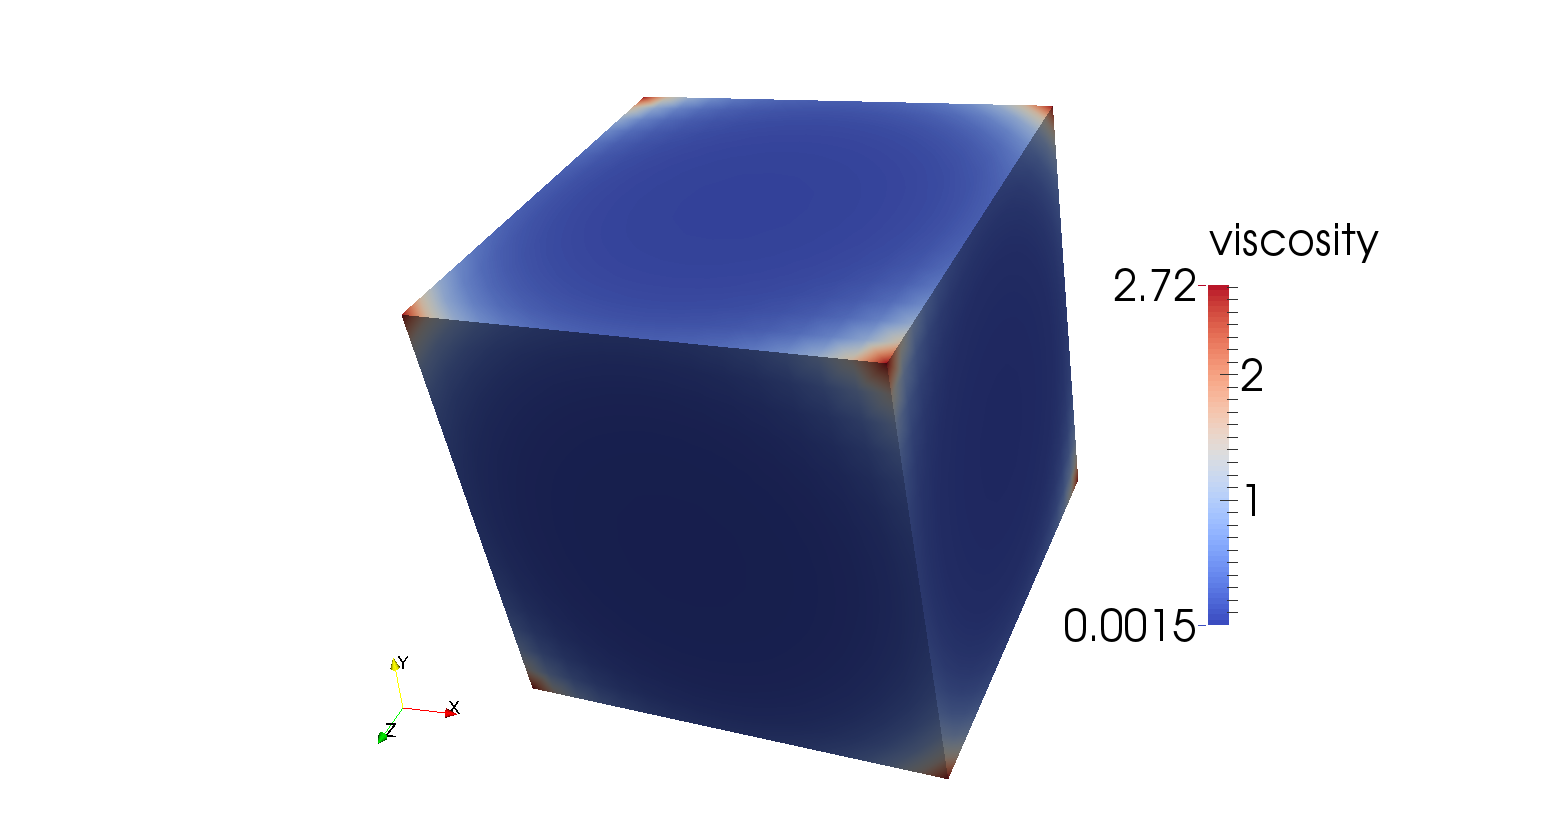
\includegraphics[width=0.48\textwidth]{cookbooks/benchmarks/burstedde/doc/viscosity.png}}%
  ~
  \subfigure[]{
    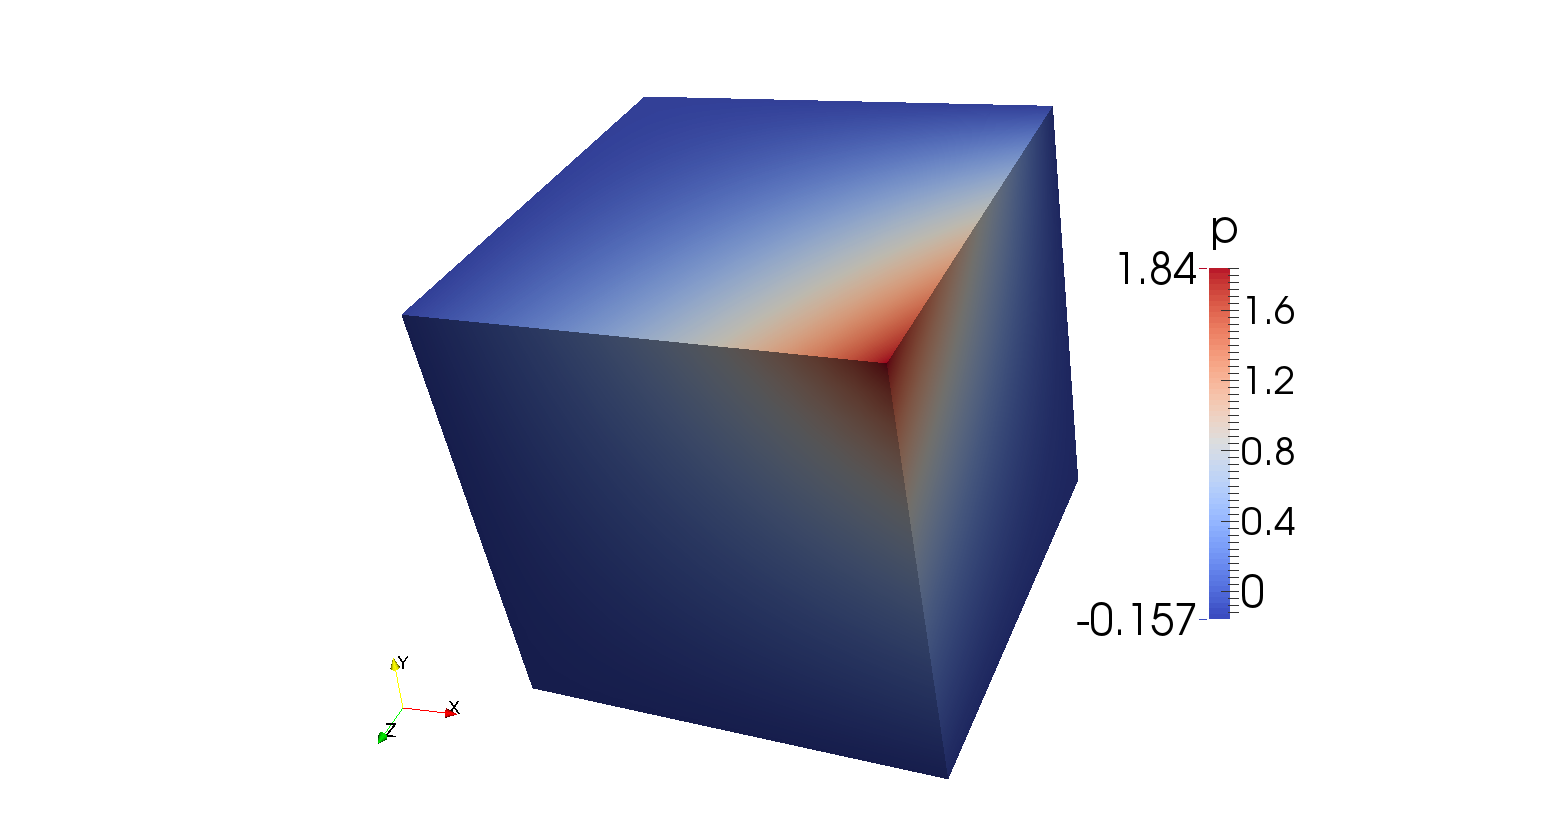
\includegraphics[width=0.48\textwidth]{cookbooks/benchmarks/burstedde/doc/pressure.png}}%
  \\
  \subfigure[]{
    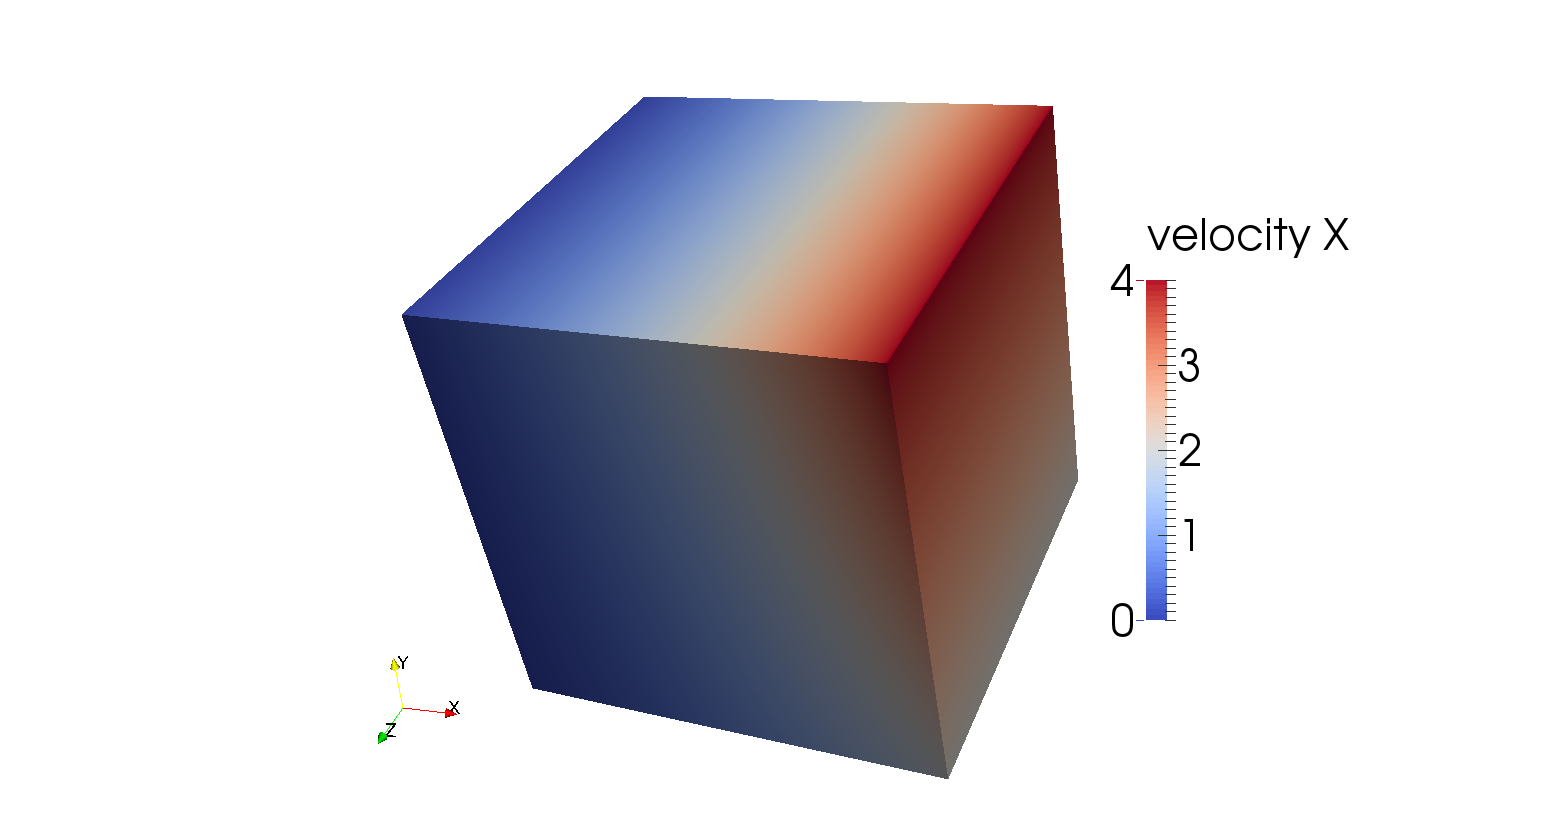
\includegraphics[width=0.48\textwidth]{cookbooks/benchmarks/burstedde/doc/velocity_x.png}}
  ~
  \subfigure[]{
    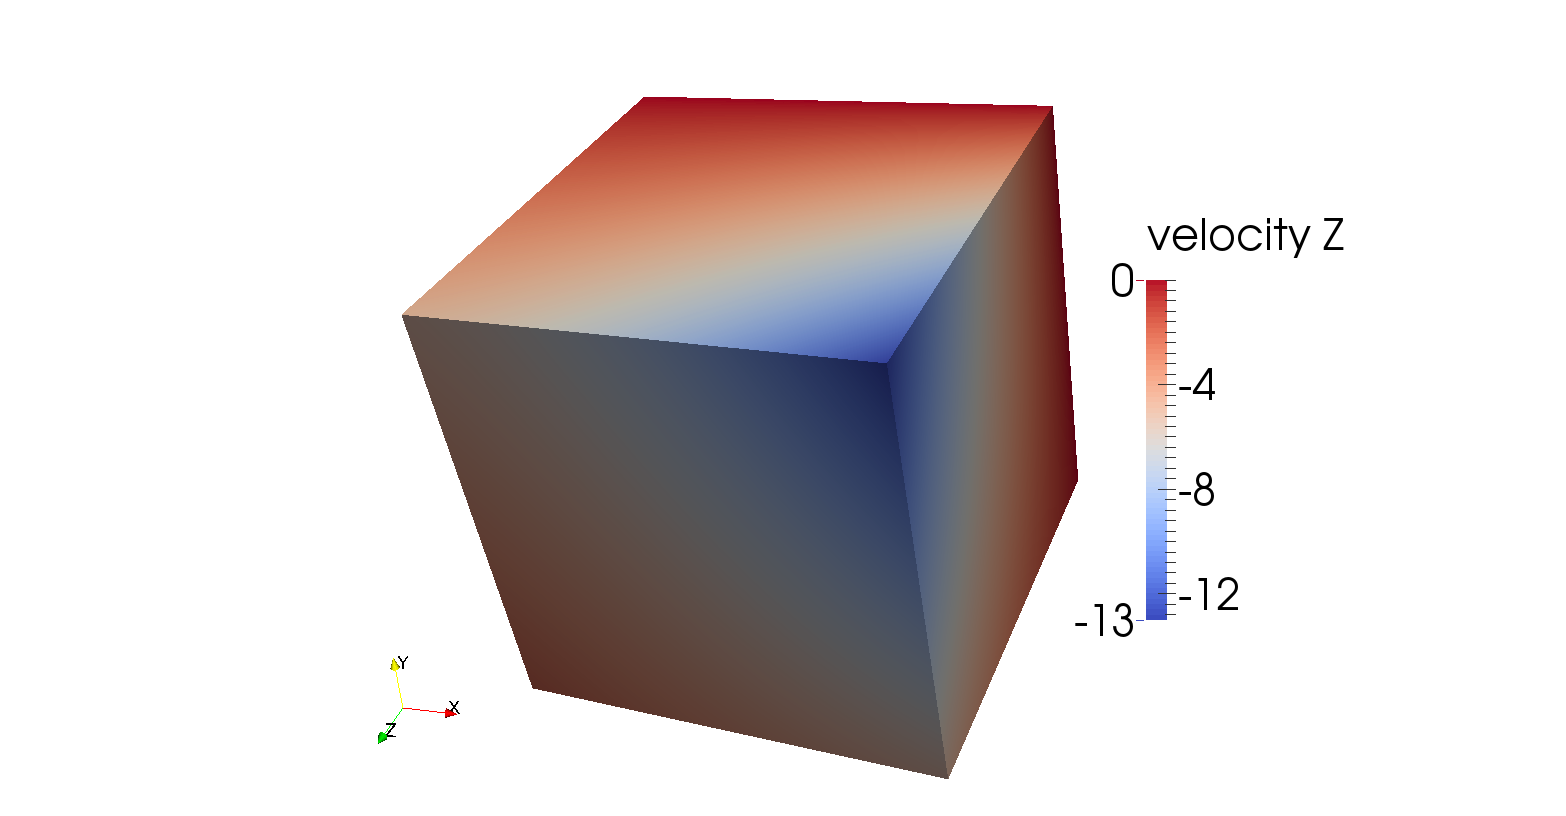
\includegraphics[width=0.48\textwidth]{cookbooks/benchmarks/burstedde/doc/velocity_z.png}}
  \caption{\it Burstedde benchmark: Results for the 3D polynomial Stokes benchmark, obtained with a resolution of $16\times 16$ elements, with $\beta = 10$.}\label{fig:burstedde-benchmark}
\end{figure}

The convergence of the numerical error of this benchmark has been analysed by
playing with the mesh refinement level in the input file, and
results can be found in Figure~\ref{errors}. The velocity shows cubic error
convergence, while the pressure shows quadratic convergence in the $L_1$ and
$L_2$ norms, as one would hope for using $Q_2$ elements for the velocity and
$Q_1$ elements for the pressure.

\begin{figure}[tbp]
  \centering
  \includesvg[width=\textwidth]{cookbooks/benchmarks/burstedde/doc/errors.svg}
  \caption{\it Burstedde benchmark: Error convergence for the 3D polynomial Stokes
    benchmark.
    \label{errors}}
\end{figure}
